\chapter{低分辨率环境下微表情识别系统}\label{chap:system}

为了将本文算法演示出来以提供更为直观的视觉效果,本章利用MATLAB GUI设计实现了一款低分辨率环境下微表情识别的展示系统。通过向该系统上传视频(或图像序列)选择合适的参数设置,输出显示对应的识别结果。

\section{需求分析}\label{sec:require}

低分辨率环境下微表情识别展示系统的主要目的是为了让研究人员能更直观的了解微表情的识别结果和对微表情数据集的理解,同时在本文中为了让文章算法更直观的呈现。介于上述目的本章将重点突出在系统可视化设计部分,将数据的输入和结果的输出作为重点,以尽量简洁的方式表达。

\section{系统设计}

一款可发布的应用程序或者算法为使使用者能够更加方便、快速地理解和使用都需要设计一个方便操作的系统,且配备相对简易的操作界面。为使本文方法更便于用户理解和学习,在本章利用MATLAB GUI设计了一款低分辨率环境下微表情识别的展示系统。

\subsection{功能设计}

通过对章节~\ref{sec:require}的分析发现该展示系统的重点为输入输出功能,如图~\ref{fig26}所示通过对需求的梳理设计了数据输入、参数设置、结果可视化和数据输出四个模块。其中在数据设置模块主要针对分类器SVM参数的设置和对分辨率的设置。前者可以通过不同参数的设置应用不同的分类器以适合不同的数据,同时也可以反映在不同参数设置下的实验对照效果。后者的分辨率设置主要针对低分辨率视频是否采用重建后图像序列设置,同样,该功能的设计考虑的是不同实验组间的对比。

在结果可视化部分尽可能多的对结果展示,包括超分辨重建效果的展示和微表情识别效果的展示。主要是通过相关指标完成,如针对超分辨重建的PSNR指标和SSIM指标,上述两个指标的结合很够有力的反应重建效果;微表情识别的指标主要为准确度的呈现和最终可能的表情类,此处将各类表情的准确度均可视化,目的是增加数据的可信度。

最后一个模块是数据输出模块,作为结果可视化的一部分该部分主要是输出一份以数据为主题的识别报告。

\begin{figure}[!htbp]
    \centering
    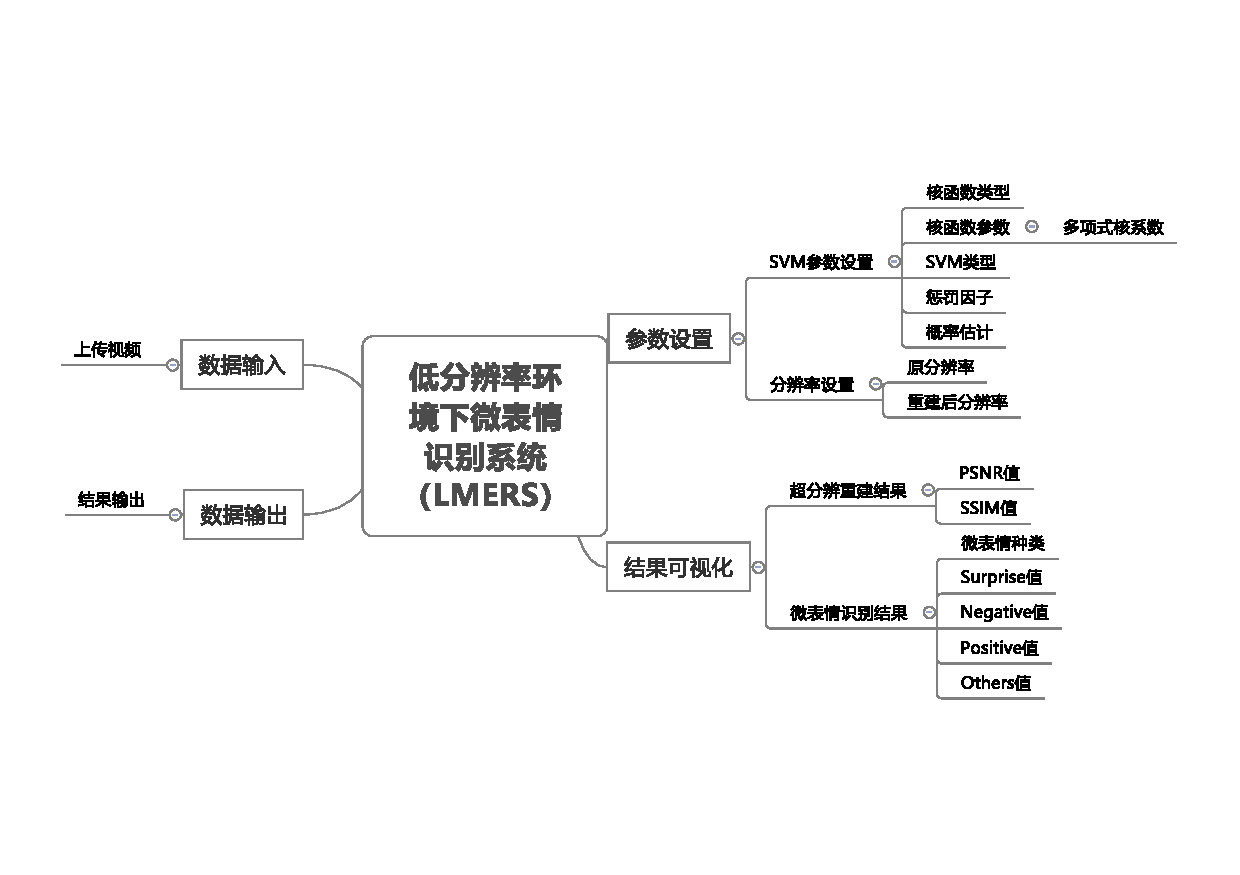
\includegraphics[width=0.85\textwidth]{MERS0}
    \caption{微表情识别系统功能结构图}
    \label{fig26}
\end{figure}

\subsection{界面设计}

MATLAB GUI是一种新型的图形用户界面开发环境,在GUI中使用者能够嵌入已经实现的仿真程序,同时还能够以动态方式将所仿真的图像化结果表现出来,具有非常好的人机交互性体验和非常实际的应用性。

在MATLAB中可以通过以下两种常见的方式来设计系统的界面:

(1)编写相应的可视化程序设计系统界面。在MATLAB中用户能够通过编写.m文件来实现系统所需要的任意界面并实现相应的功能。

(2)使用可视化的界面利用控件设计系统界面。相对直接通过编写代码生成.m文件进行界面设计而言,GUI中控件的使用为用户提供了一种更为方便高效的方法,即guide方法,但同时其也表现出一定的局限性。用户只需在MATLAB的命令框中输入guide命令,系统会立即自动生成后缀名分别为.fig和.m的两个文件,其中.fig是资源文件,.m文件则包含界面初始化的相关代码,通过guide方法,用户能够将所需要的控件直接放到界面区域并调整相应布局。

在本章的系统设计中采用了两者结合的方式来制作演示系统,主要原因是guide方法提供的控件有限,不能完全满足界面设计的需要。

\begin{figure}[!htbp]
    \centering
    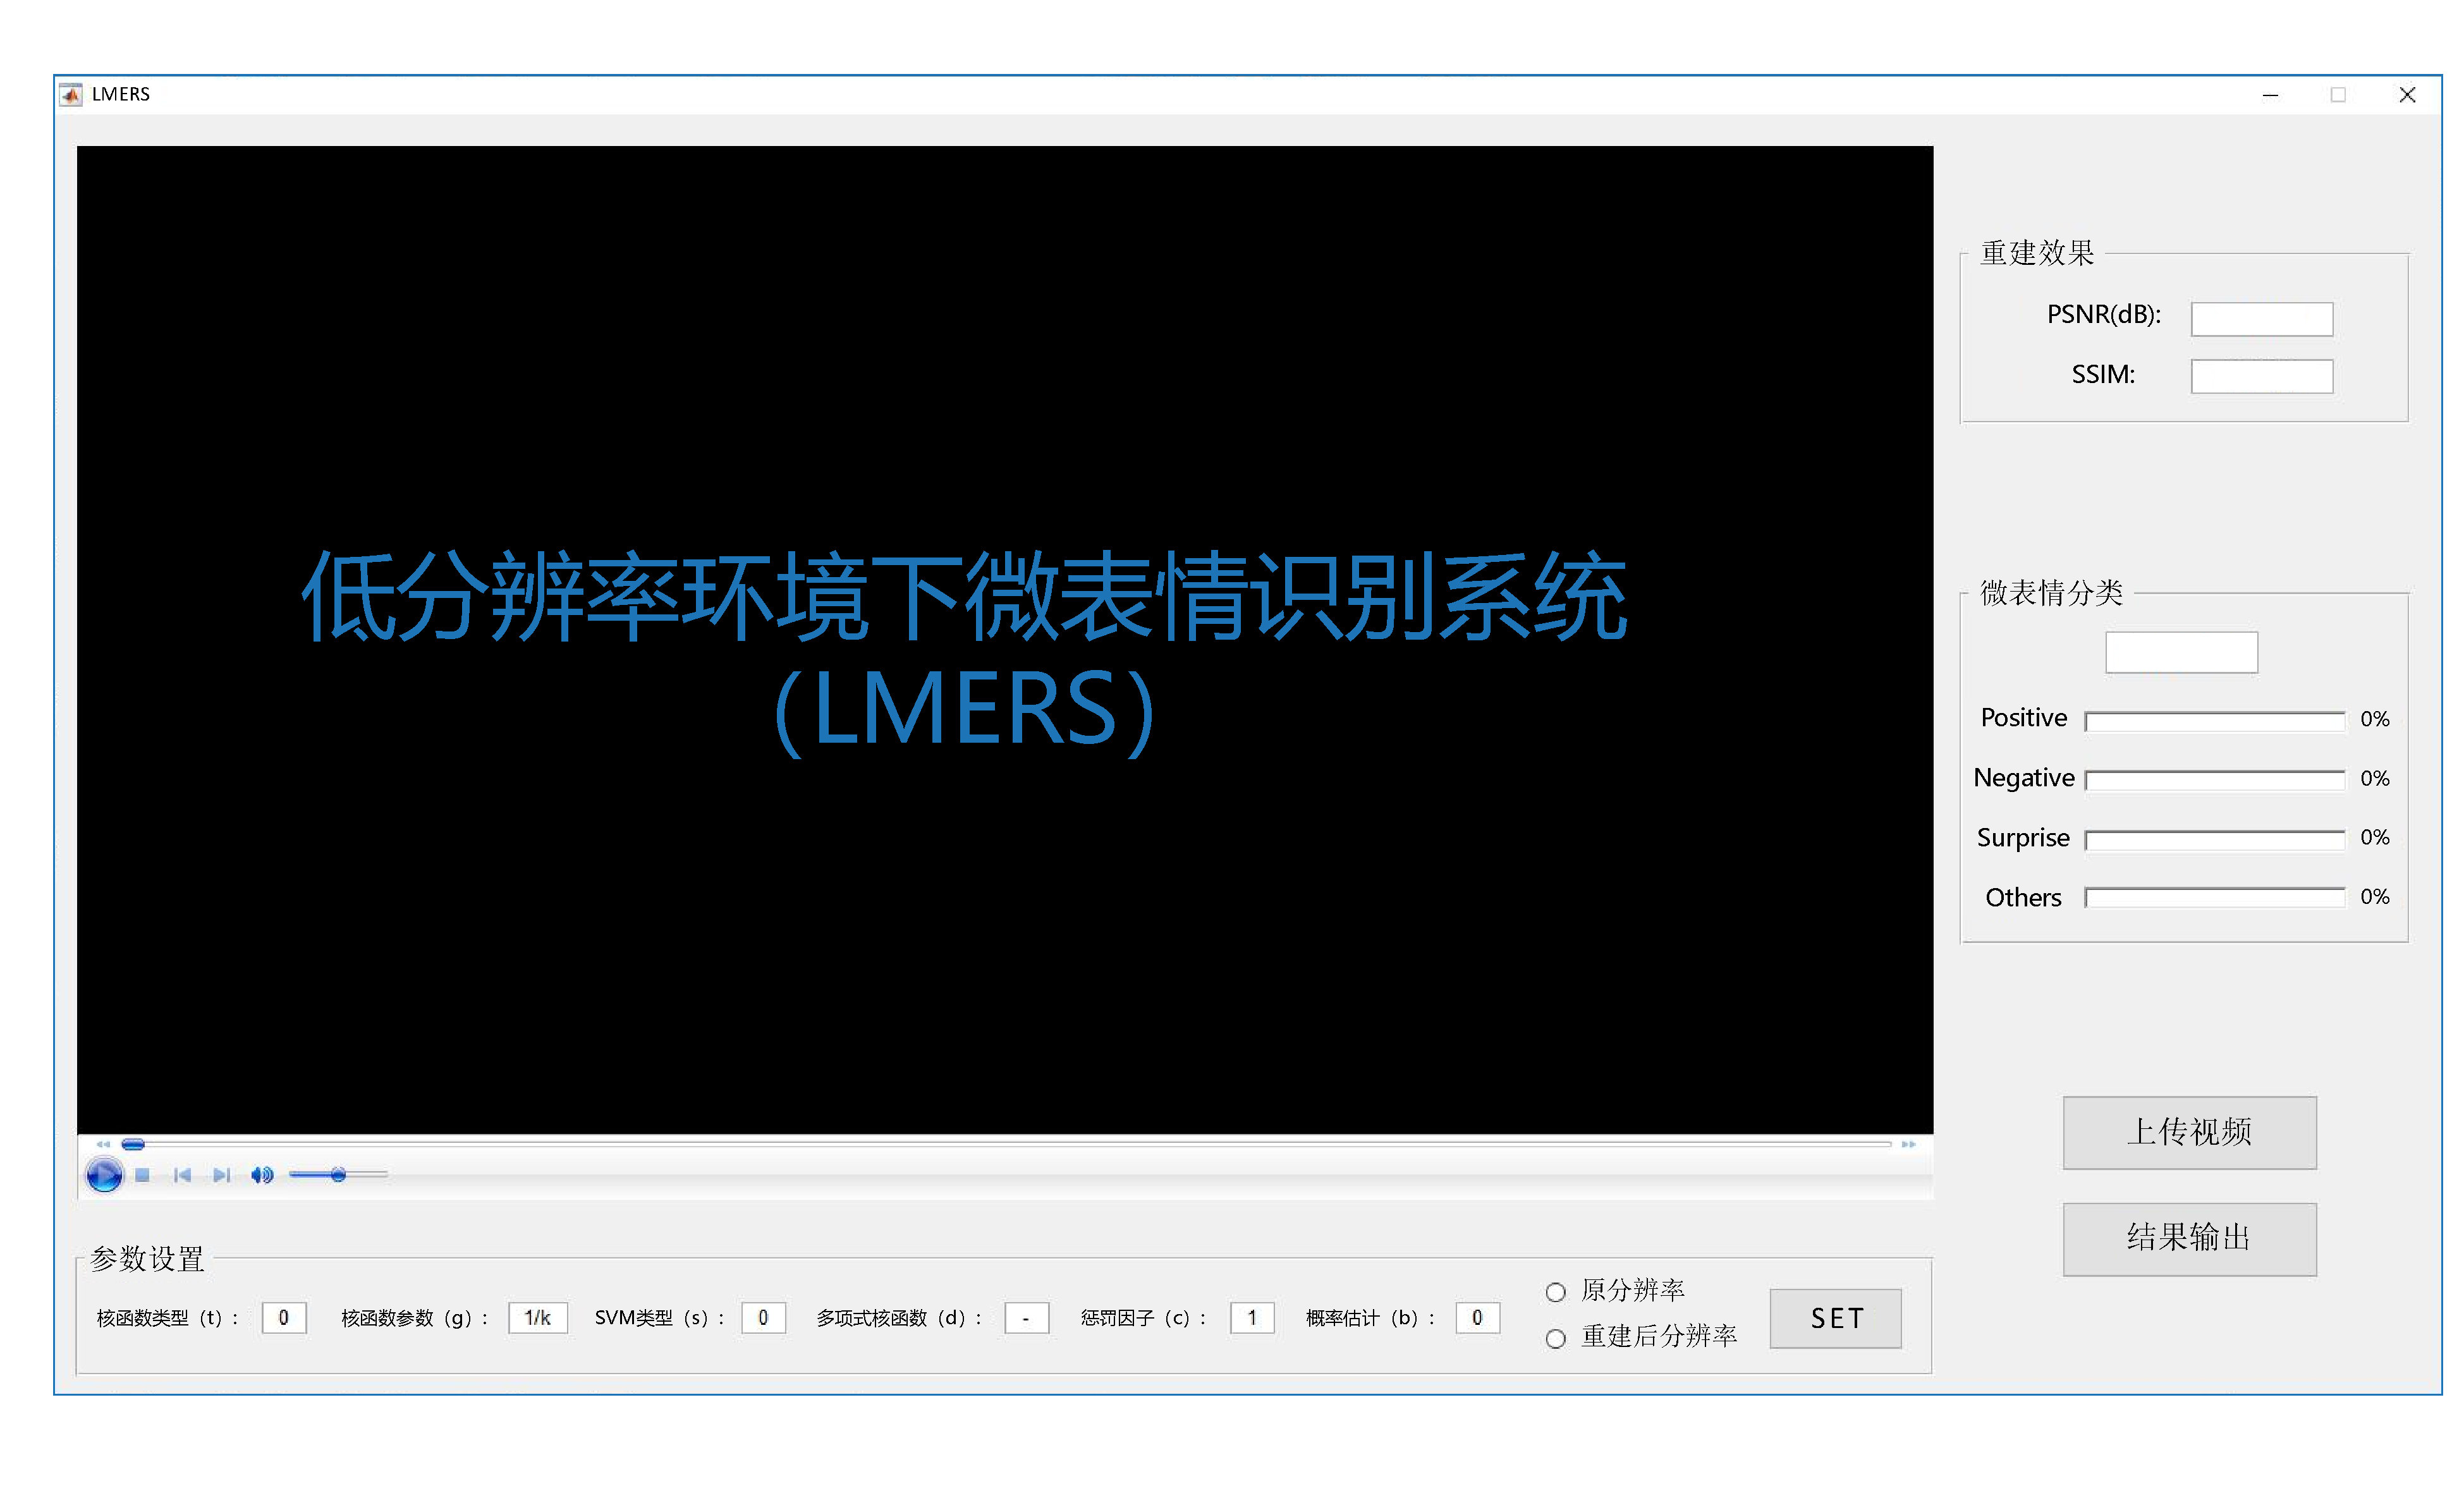
\includegraphics[width=0.9\textwidth]{MERS1}
    \caption{低分辨率环境下微表情识别系统}
    \label{fig27}
\end{figure}

如图~\ref{fig27}所示本章设计的演示系统的界面包括4个部分:左上方的视频播放界面、右上方的结果可视化界面、左下方的参数设置界面和右下方的数据输入输出界面。

点击“立即体验”直接跳转到修复界面,如图5-2所示;点击“系统说明”可以查看该系统的主要功能相关介绍,如图5-3所示;点击“关于”可以查看该系统设计的相关信息,如图5-4所示;点击“退出”会出现图5-5的提示窗,点击“Yes”退出演示系统,点击“No”或“Cancel”则关闭提示窗并回到主界面。

修复界面下总共包括“读取图像”、“图像修复算法”、“保存修复结果”和“退出”四个模块,各个模块的功能将在下文中介绍。



\subsection{操作样例}

\begin{figure}[!htbp]
    \centering
    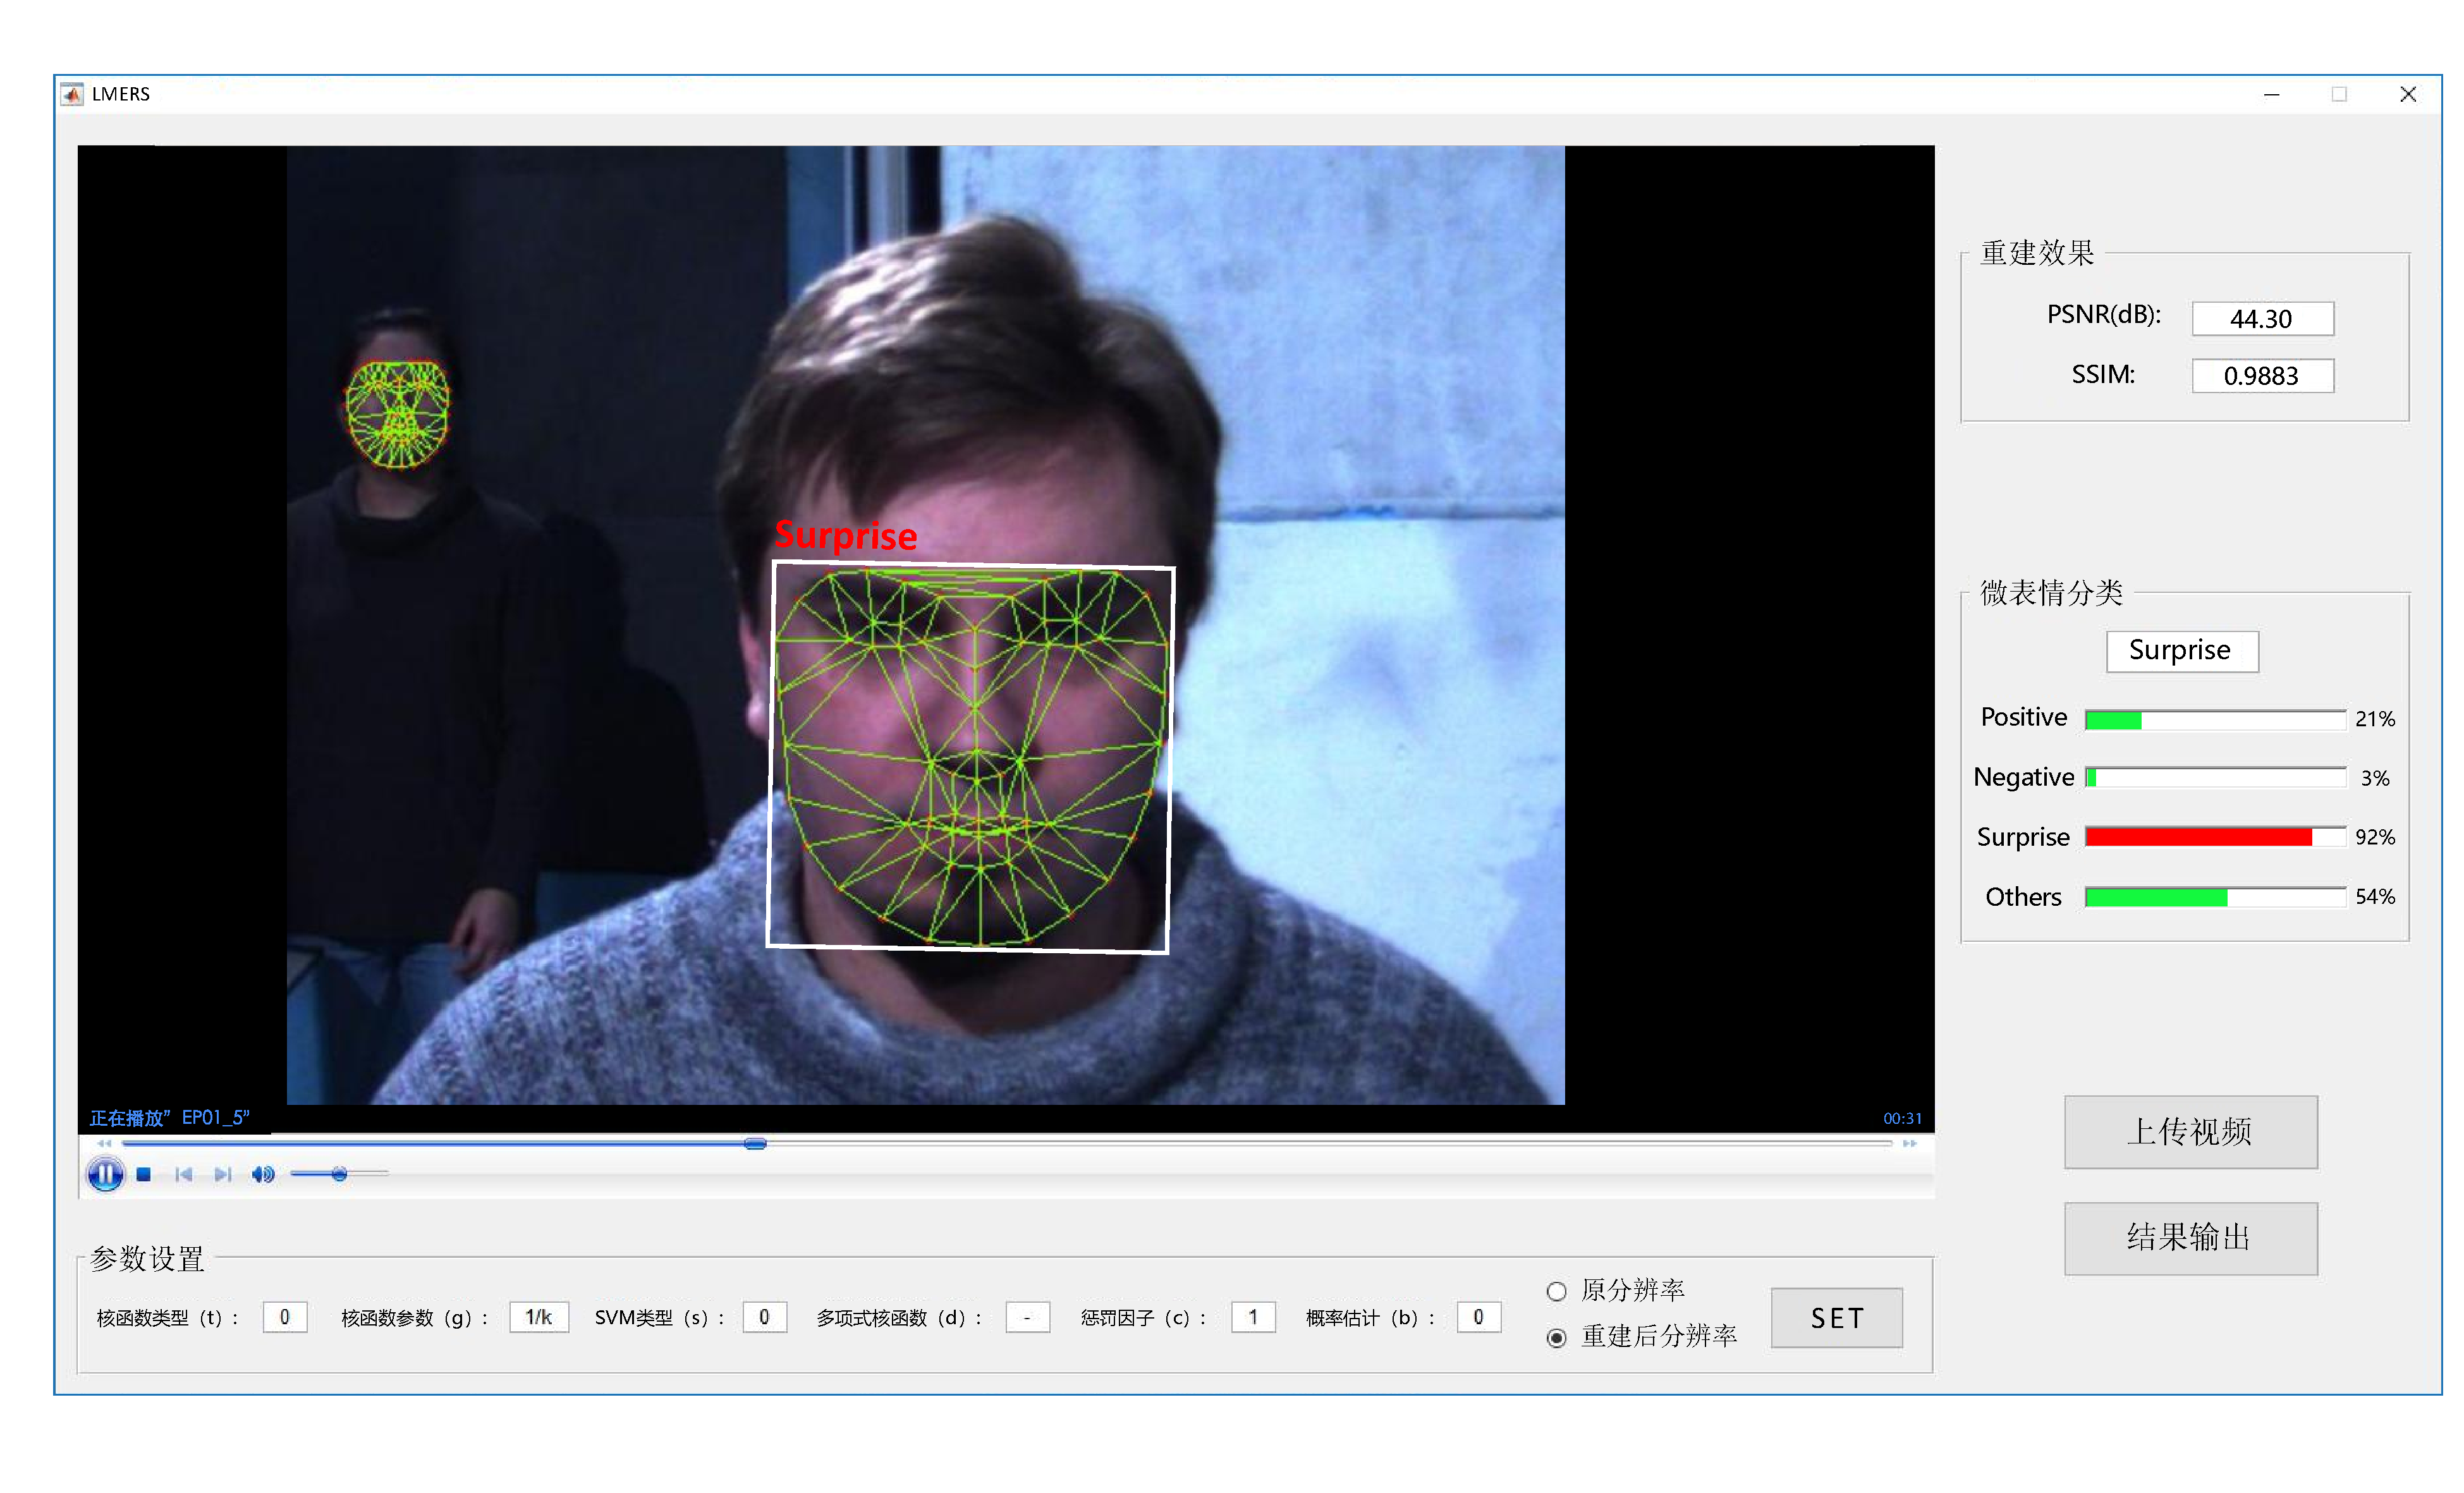
\includegraphics[width=0.9\textwidth]{MERS2}
    \caption{低分辨率环境下微表情识别样例}
    \label{fig28}
\end{figure}

\section{本章小结}

为了使本文算法演示起来更加方便简单,设计了一款低分辨率环境下微表情识别效果展示系统,在这款系统中用户可以通过上传视频,并通过设置不同的参数对不同的视频片段分析并输出显示对应的识别结果。
